\chapter{Introduction}
The purpose of this project is to use generative art techniques to explore the
spaces created by the works of the artist \emph{Darrell Viner (1947-2001)}. Viner's work
included movement, sound, and light, and though primarily working with
sculpture, he produced a series of pen plotter drawings. These drawings have
been called pioneering works in the field of computer art \citep{viner_bio}.

\begin{figure}[H]
    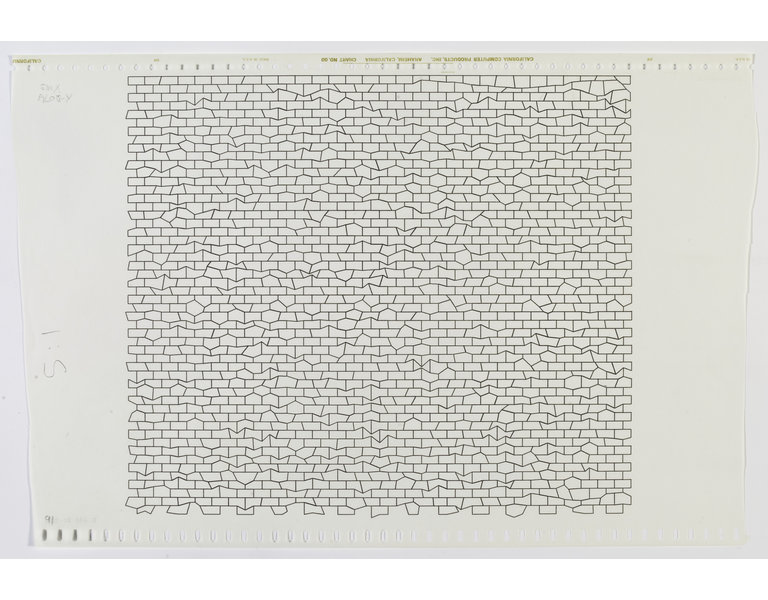
\includegraphics[scale=0.4]{viner1}
    \centering
    \caption{\emph{Darrell Viner, Untitled (1974)} \copyright Victoria and Albert Museum, London.}
\end{figure}

Generative art is any art that is created with some system that produces
an output, it can either be art that is completed by hand (e.g. a painting)
with some system, or a stochastic process. Or, more commonly art that is
generated by a computer program with some initial parameters.

The project will incorporate graphics and sound to create software that can be
used to explore the landscapes present in Viner's works. The major problem that
needs to be solved in this project is creating an interface that allows the user
to interact meaningfully with the program and a set of parameters that might be
changed to produce an image. As an extension of the graphics, a musical
component will also be produced, this is less about Viner and more about
creating a piece of art that stands apart from his work, but is still influenced
and adds to the visual aspect.

\section{Problem Overview}
Viner spoke about his work being like a ``townscape/landscape'': 
``Basically it is a self-generating program which depends on the start
conditions. Thus, by altering parameters of the program, changes in the
final image can be achieved. Currently, I am after images which have the feel and
scale of townscapes/landscapes. The program is modified depending upon whether I
consider the images to be working or not: the program has become my personal
aesthetic.'' \cite{viner_artiststatement}

These parameters may for example control the spacing of the grid, the
displacement of each point, the number of vertices in a shape, so on. These
parameters should be able to be changed to create some sort of `landscape' or
`topography' that the user can explore through manipulating the program
affecting both the entire grid and single points within it. Later on, I will
detail methods for users being able to manipulate the parameters and
considerations that need to be made concerning usability.

\begin{figure}[H]
    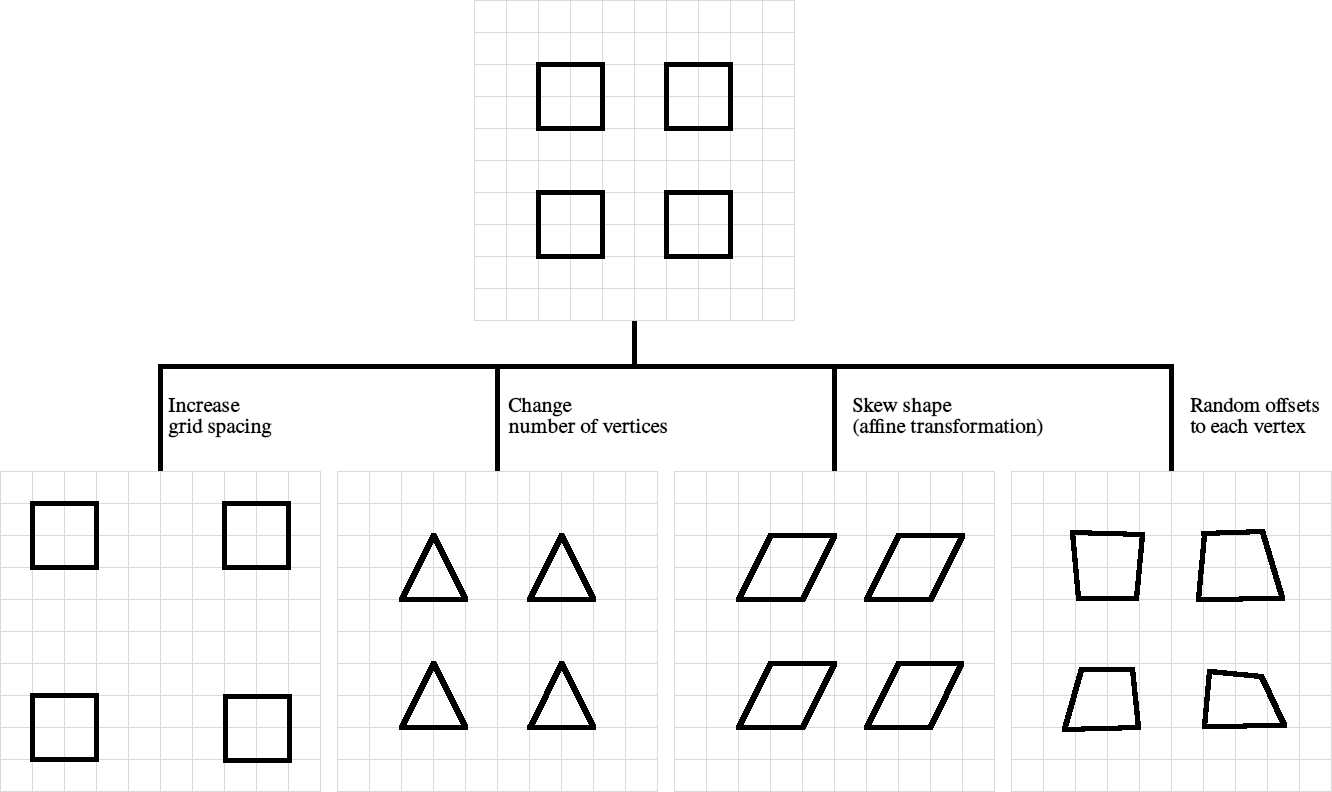
\includegraphics[width=\textwidth]{parametercomparison}
    \caption{Example of changing parameters from an initial state}
\end{figure}

The program should allow for a user to generate such images and recall them
later. Ideally, the program should be more than just a show of the potential
configurations of Viner's work and itself be a unique experience for the user
and work to create a dialogue with the original work and contextualise the
user's understanding of his work.

Users of this program may be for example artists, art scholars, museum guests,
museum curators. Each of these has different goals; the artist may be seeking
to understand the work and find inspiration in it, the art scholar may be
looking for an extended context to the work to help comprehend the thought
process Viner used and the relationships between each piece. The museum guest may be
at an exhibition (perhaps a virtual one) of Viner's work and have this presented
as a piece of work that helps them understand the spaces that are explored by
the work. A curator might be evaluating the program for display alongside
Viner's work.

\section{Aim}
Using the idea of a virtual museum exhibition of Viner's work: this could be
presented alongside a collection of images to show the relationships between
each image where in a physical museum this may be able to be explained through
the placement of the images in the physical space, online this is harder to
convey with just a gallery on a web page.

The user should be engaged with the program and be able to become engaged with
using it with minimal instruction. Through using the program the user should
understand the concept of the `landscape' described previously. To show the
relationships between images and for the user to be able to explore these a
method for seeing previous states of the program should be provided.

To create the graphics, a system needs to be created to display polygons in a
grid of which each vertex can be offset separately. The calculation of these
offsets and the number of vertices in each polygon is what will convey the idea
of the `landscape'. These offsets need to be calculated in a way that is
repeatable so that the user can revisit parts of the `landscape' both in the
session and between different sessions. This will require the development of a
set of tools to create an aesthetically pleasing image.

The audio component extends to the idea of an exhibit; a museum version of this
would have a pair of headphones that the user can wear which would help isolate the
piece of art from the rest of the exhibit. In the case of people accessing the
piece online the same applies, with audio they can be more immersed in the art.
Also, since the audio relates to the graphics on the screen, it can help users
navigate the `landscape' by providing cues.

Less focused on the exhibition example, through this report techniques that
apply to other works of generative art and music will be outlined. The idea is
that they may be reused. In this sense, the program also is for artists wishing
to create pieces of work, and by presenting these techniques may use them for
their ends; therefore, code should be reusable and understandable.

\section{Objectives}
% These should be testable objectives
\begin{itemize}
    \item To create a program that allows the user to experience the works of
        Viner through the manipulation of parameters in a way that enables
        exploration and recall. 
    \item Create an interface that allows users to navigate generated spaces.
    \item Create an audio component that works in tandem with the graphical aspect
        of the program to aid navigation and provide an extra layer to the
        experience.
    \item Create a system such that users can recall a state they were
        in, and find it again.
    \item Create a system such that users can download and upload the collection
        of states as described in the previous objective.
    \item Develop a catalogue of techniques to be used in generative art and
        music, and to evaluate each for relevance to the project.
\end{itemize}

\section{Deliverables}
An application written using \verb|p5js| that should allow the user to explore a
landscape, generated to feel like Viner's work. This application should be
friendly to use and will include both graphics and sound. The feeling of some
sort of topography should be conveyed and the visual should look similar to
Viner's work. The audio will help the user navigate the space and correspond to
what is on the screen graphically in some way.

The application should work in the browser, and be as compatible as possible
with different screen sizes and web technologies, libraries allowing. Thus, not
requiring hosting with a web browser, allowing for flexibility.

The structure of the final product will consist of three main components: the
graphics which consist mainly of the grid; the audio which will be changed by the
parameters that generate the graphics; and the history / recall part which will
deal with data structures associated with saving the state of the parameters.

The graphics component is what will utilise the \verb|p5js| library, although it
will also be utilised in the history component. The audio part will use the
\verb|Tone.js| library. This is represented by the first five objectives
(deliverables 1-5).

Also presented are two code examples of techniques used in this project that use
p5js, in a \verb|report-demos| directory. This is represented by the last
objective (deliverable 6).

The final program will be hosted on \verb|github.io| and sent as a deliverable
(deliverable 7).

\section{Plan}
Being that this project is exploratory, an iterative approach to
development makes sense, with small prototypes being created, explored, and
built on quickly. As such I have allocated time for ideas to be developed in.

To start I will learn about \verb|processing|, a library for Java which is an
artist-focused library for graphics and audio. Since my tutor's previous work
was written in processing, there is already some groundwork complete to build
on. I will then switch to \verb|p5js|, a JavaScript library based on
\verb|processing| that is an offshoot and works in the browser using JavaScript.
This switch will not take much time at all due to the program logic being
identical. \verb|p5js| in the browser has the advantage of working with other
JavaScript libraries well (such as \verb|Tone.JS|, the audio library I will be
using) as well as having the flexibility that comes with HTML and CSS for the
user interface.

\begin{center}
    \begin{ganttchart}[
        vgrid,
        y unit title=0.4cm,
        y unit chart=0.4cm,
        x unit=0.4cm,
        milestone label font = \tiny,
        title label font=\tiny,
        group label font=\tiny,
        bar label node/.style={align=right,font=\tiny, anchor=east},
        ]{1}{24}
        \gantttitle{Week}{24}\\
        \gantttitlelist{1,...,24}{1} \\
        \ganttgroup{Semester 1}{1}{12}\\
        \ganttmilestone{Initial report hand-in}{12}\\
        \ganttgroup{Semester 2}{13}{24}\\
        \ganttmilestone{Progress meeting}{19}\\
        \ganttmilestone{Final hand-in}{24}\\
        \ganttbar{Learning processing}{1}{2} \\
        \ganttbar{Exploring audio ideas}{3}{4} \ganttbar{}{7}{9} \\
        \ganttbar{Exploring polygon drawing}{5}{9} \\
        \ganttbar{Creating demo with grid and audio}{6}{7} \\
        \ganttbar{Final PoC for init report}{9}{12} \\
        \ganttbar{Writing init report}{1}{12}\\
        \ganttbar{Switch to p5js}{13}{13}\\
        \ganttbar{Implement synth and audio}{13}{16} \ganttbar{}{19}{21}\\
        \ganttbar{Implement history}{14}{18}\\
        \ganttbar{Noise implementation}{18}{18}\\
        \ganttbar{General graphical work}{19}{20}\\
        \ganttbar{Create final UI}{20}{21}\\
        \ganttbar{User Testing}{22}{22}\\
        \ganttbar{Write final report}{12}{24}
    \end{ganttchart}
\end{center}

I will use \verb|git| for version control, during development commits will be
pushed to a private GitHub repository which, when complete will be made public
and the \verb|github.io| website-hosting feature will allow for the project to
be available in full on GitHub for user testing and marking.

\section{Risk Mitigation}
Since this project is not dependent on external factors, there aren't a lot of risks to
consider.

If the project had relied on access to the art directly, the COVID-19 pandemic
would have affected it, but we mitigated this risk by setting the scope of the
project to not include access to the art.

Another risk in this project is scope creep; since the project is artistic it
can be easy to have lots of ideas whilst losing the original focus. To combat
this I will set specific objectives and deliverables and reach those before
exploring any further options.
